\documentclass{article}
\usepackage{tikz}
\usetikzlibrary{arrows.meta}
\usepackage{xcolor}
\definecolor{skyblue}{RGB}{135,206,250}
\usepackage{listings}
\usepackage{graphicx}
\title{Graphs with Tikz}
\author{Credit: https://github.com/HasibLearntogrow/LatexPractice}
\begin{document}


	\maketitle
	\tableofcontents
	\clearpage
\lstset{
 language=[LaTeX]TeX,           % Set LaTeX language
 basicstyle=\ttfamily\footnotesize,
    keywordstyle=\color{blue},
    stringstyle=\color{red},
    commentstyle=\color{green!60!black},
    numbers=left,
    numberstyle=\tiny\color{gray},
    stepnumber=1,
    numbersep=10pt,
    frame=single,
    showstringspaces=false,
    breaklines=true,
    tabsize=2      
}
	
	\section{Nodes:}
		\subsection{Normal Node:}
			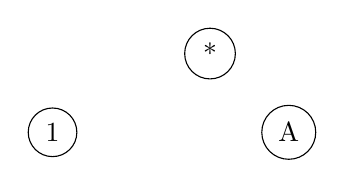
\begin{tikzpicture}
				\node(1) at (0,0) [circle,draw]{1};
				\node(2) at (2,1) [circle,draw]{*};
				\node(3) at (3,0)[circle,draw]{A};
			\end{tikzpicture}
			
		\subsection{Normal Nodes with various shapes:}
			\begin{tikzpicture}
				\node(1) at (0,0)[circle, draw]{1};
				
				\node(2) at (5,0)[draw]{2};
			\end{tikzpicture}
			
		\subsection{Normal Nodes with filled color and face color:}
		% For Fill color: \node(serial_of_node) at(x,y)[circle,color_name,draw]{name_of node}
	%For Face colore:  \node(serial_of_node) at(x,y)[circle,fill=color_name,draw]{name_of node}
	% For face and Fill at time: \node(serial_of_node) at(x,y)[circle,color_name,fill=color_name,draw]{name_of node}
			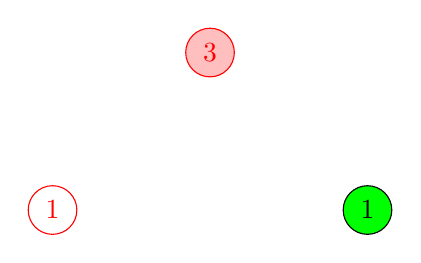
\begin{tikzpicture}
				\node(1) at (0,0) [circle,red,draw]{1};
				\node(2) at (4,0) [circle,fill=green,draw]{1};
				\node(3) at (2,2)[circle,red,fill=pink,draw]{3};
			\end{tikzpicture}
			
		\subsection{A solid node with outside title:}
		%we can use: label=left/right/below/above
	% for size= inner spp= valuept
	%For Text color: text=color_name
			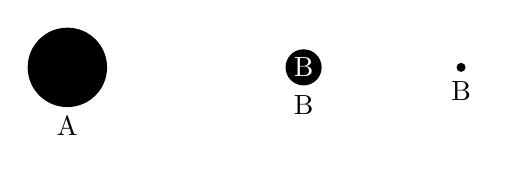
\begin{tikzpicture}
				\node(1) at (0,0)[circle,fill=black,text=white,inner sep=10pt,label=below:A,draw]{};
				\node(2) at (3,0)[circle,fill=black,text=white,inner sep=1pt,label=below:B,draw]{B};
				\node(3) at (5,0)[circle,fill=black,text=white,inner sep=1pt,label=below:B,draw]{};
				
			\end{tikzpicture}
			
%-------------------------------------------------------------------------------------------------			
	\section{Edges:}
		\subsection{Normal edge between two or more nodes:}
			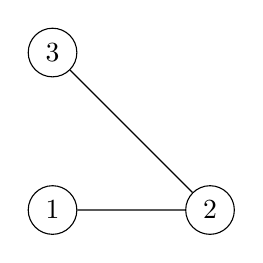
\begin{tikzpicture}
				\node(1) at (0,0)[circle,draw]{1};
				\node(2) at (2,0)[circle,draw]{2};
				\node(3) at (0,2)[circle,draw]{3};
				\draw(1) to (2) -- (3);		
			\end{tikzpicture}
			
		\subsection{Normal edge with arrow and color between two or among more nodes:}
			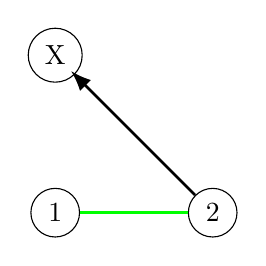
\begin{tikzpicture}
				\node(1) at (0,0)[circle,draw]{1};
				\node(2) at (2,0)[circle,draw]{2};
				\node(3) at (0,2)[circle,draw]{X};
				\draw[-,very thick,green](1)--(2);	
				%\usetikzlibrary{arrows.meta}
				\draw[->, >=Latex, line width=1pt, shorten >=-2pt](2) to (3);	
			\end{tikzpicture}
			
		\subsection{Curved edge with arrow between two or among more node:}
		%Create: upward curved edge:  \draw[->, bend left=angle] (starting_node) to (ending_node);
	%Create: downward curved edge:  \draw[->, bend right=angle] (starting_node) to (ending_node);
			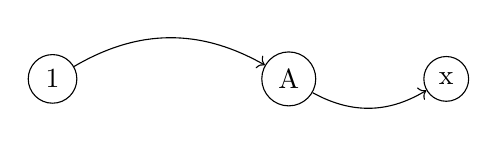
\begin{tikzpicture}
				\node(1) at (0,0)[circle,draw]{1};
				\node(2) at (3,0) [circle,draw]{A};
				\node(3) at (5,0)[circle ,draw]{x};
				\draw[->,bend left=30](1) to (2);	
				\draw[->,bend right=30](2) to (3);			\end{tikzpicture}			
			
		\subsection{Self loop in any node:}
			\begin{tikzpicture}
				\node(1) at (0,0)[circle,draw]{1};
				\draw[->,loop above](1) to (1);	
				\node(2) at (5,0)[circle,draw]{2};
				\draw[->,loop right](2) to (2);	
			\end{tikzpicture}
			
%-------------------------------------------------------------------------------------------------			
	\section{Practice:}
		\subsection{Practice 01:}
			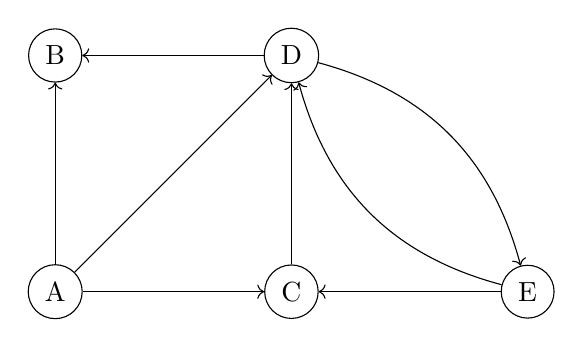
\begin{tikzpicture}
				\node(B) at (0,0)[circle,draw]{B};
				\node(D) at (3,0)[circle,draw]{D};
				\node(A) at (0,-3)[circle,draw]{A};
				\node(C) at (3,-3)[circle,draw]{C};
				\node(E) at (6,-3)[circle,draw]{E};
				
				\draw[->] (A) to (B);
				\draw[->] (D) to (B);
				\draw[->] (A) to (D);
				\draw[->] (A) to (C);
				\draw[->] (E) to (C);
				\draw[->] (C) to (D);
				\draw[->, bend left=30] (D) to (E);
				\draw[->, bend left=30] (E) to (D);
			\end{tikzpicture}
			
		\subsection{Practice 02:}
			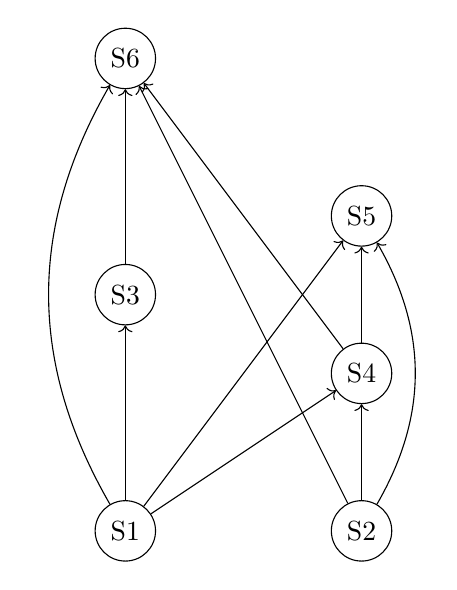
\begin{tikzpicture}
				\node(s6) at (0,0)[circle,draw]{S6};
				\node(s3) at (0,-3)[circle,draw]{S3};
				\node(s1) at (0,-6)[circle,draw]{S1};
				\node(s5) at (3,-2)[circle,draw]{S5};
				\node(s4) at (3,-4)[circle,draw]{S4};
				\node(s2) at (3,-6)[circle,draw]{S2};
				
				\draw[->] (s1) to (s3);
				\draw[->] (s1) to (s4);
				\draw[->] (s1) to (s5);
				\draw[->] (s2) to (s6);
				\draw[->] (s4) to (s6);
				\draw[->] (s3) to (s6);
				\draw[->] (s2) to (s4);
				\draw[->] (s4) to (s5);
				\draw[->, bend left = 30] (s1) to (s6);
				\draw[->, bend right = 30] (s2) to (s5);
				
			\end{tikzpicture}
			
		\subsection{Practice 3:}
\begin{lstlisting}
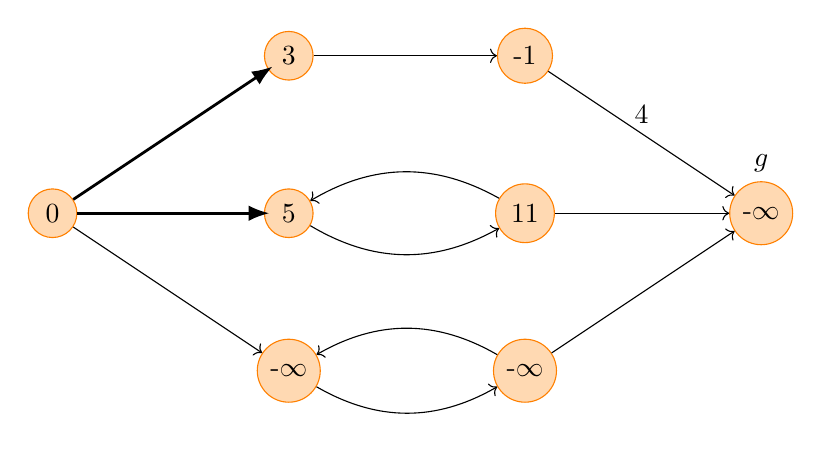
\begin{tikzpicture}
	\node(0) at (0,0)[circle,orange,fill= orange!30,text=black,draw]{0};
	\node(3) at (3,2)[circle,orange,fill= orange!30,text=black,draw]{3};
	\node(5) at (3,0)[circle,orange,fill= orange!30,text=black,draw]{5};
	\node(i1) at (3,-2)[circle,orange,fill= orange!30,text=black,draw]{-$\infty$};
	\node(-1) at (6,2)[circle,orange,fill= orange!30,text=black,draw]{-1};
	\node(11) at (6,0)[circle,orange,fill= orange!30,text=black,draw]{11};
	\node(i2) at (6,-2)[circle,orange,fill= orange!30,text=black,draw]{-$\infty$};
	\node(i3) at (9,0)[circle,orange,fill= orange!30,text=black,label=above:$g$,draw]{-$\infty$};
%\usetikzlibrary{arrows.meta}
	\draw[->, >=Latex, line width=1pt, shorten >=-2pt] (0) to (3);
	\draw[->, >=Latex, line width=1pt, shorten >=-2pt] (0) -- (5);
	\draw[->] (0) to (i1);
	\draw[->] (3) to (-1);
	\draw[->, bend right =30] (5) to (11);
	\draw[->,bend right =30] (11) to (5);
	\draw[->, bend right =30] (i1) to (i2);
	\draw[->,bend right =30] (i2) to (i1);
	\draw[->] (-1) to  node[midway, above]{4}(i3);
	\draw[->] (11) to (i3);
	\draw[->] (i2) to (i3);
				
\end{tikzpicture}
\end{lstlisting}
			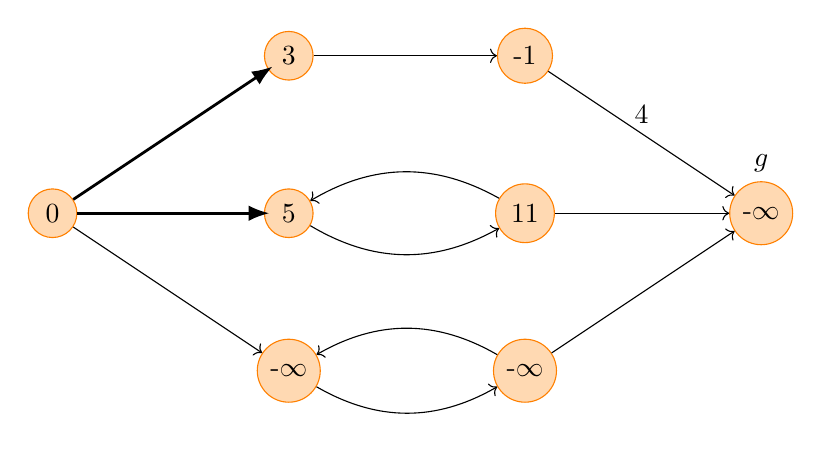
\begin{tikzpicture}
				\node(0) at (0,0)[circle,orange,fill= orange!30,text=black,draw]{0};
				\node(3) at (3,2)[circle,orange,fill= orange!30,text=black,draw]{3};
				\node(5) at (3,0)[circle,orange,fill= orange!30,text=black,draw]{5};
				\node(i1) at (3,-2)[circle,orange,fill= orange!30,text=black,draw]{-$\infty$};
				\node(-1) at (6,2)[circle,orange,fill= orange!30,text=black,draw]{-1};
				\node(11) at (6,0)[circle,orange,fill= orange!30,text=black,draw]{11};
				\node(i2) at (6,-2)[circle,orange,fill= orange!30,text=black,draw]{-$\infty$};
				\node(i3) at (9,0)[circle,orange,fill= orange!30,text=black,label=above:$g$,draw]{-$\infty$};
%\usetikzlibrary{arrows.meta}
				\draw[->, >=Latex, line width=1pt, shorten >=-2pt] (0) to (3);
				\draw[->, >=Latex, line width=1pt, shorten >=-2pt] (0) -- (5);
				\draw[->] (0) to (i1);
				\draw[->] (3) to (-1);
				\draw[->, bend right =30] (5) to (11);
				\draw[->,bend right =30] (11) to (5);
				\draw[->, bend right =30] (i1) to (i2);
				\draw[->,bend right =30] (i2) to (i1);
				\draw[->] (-1) to  node[midway, above]{4}(i3);
				\draw[->] (11) to (i3);
				\draw[->] (i2) to (i3);
				
			\end{tikzpicture}
			
		\subsection{Practice 04:}
\begin{lstlisting}
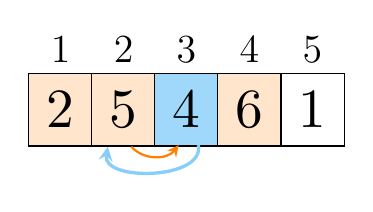
\begin{tikzpicture}
	\node(2) at (0,0)[text=black,fill=orange!20,label=\Large1,draw,scale=2]{2};
	\node(5) at (0.8,0)[text=black,fill=orange!20,label=\Large2,draw,scale=2]{5};
	\node(4) at (1.6,0)[text=black,fill=skyblue!80,label=\Large 3,draw,scale=2]{4};
	\node(6) at (2.4,0)[text=black,fill=orange!20,label=\Large 4,draw,scale=2]{6};
	\node(1) at (3.2,0)[text=black,label=\Large 5,draw,scale=2]{1};
			
	\draw[->,>=stealth,very thick,skyblue,bend left=100](1.75,-0.45) to (0.6,-0.47);
	\draw[->,>=stealth,thick,orange,bend angle=50,bend right](0.9,-0.47) to (1.5,-0.45); 
\end{tikzpicture}
\end{lstlisting}

		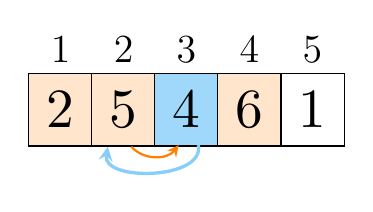
\begin{tikzpicture}
			\node(2) at (0,0)[text=black,fill=orange!20,label=\Large1,draw,scale=2]{2};
			\node(5) at (0.8,0)[text=black,fill=orange!20,label=\Large2,draw,scale=2]{5};
			\node(4) at (1.6,0)[text=black,fill=skyblue!80,label=\Large 3,draw,scale=2]{4};
			\node(6) at (2.4,0)[text=black,fill=orange!20,label=\Large 4,draw,scale=2]{6};
			\node(1) at (3.2,0)[text=black,label=\Large 5,draw,scale=2]{1};
			
			\draw[->,>=stealth,very thick,skyblue,bend left=100](1.75,-0.45) to (0.6,-0.47);
			\draw[->,>=stealth,thick,orange,bend angle=50,bend right](0.9,-0.47) to (1.5,-0.45); 
		\end{tikzpicture}
\pagebreak
		\subsection{Practice 05:}
\begin{lstlisting}
\begin{tikzpicture}
	\node(0) at (0,0)[text=black,fill=skyblue!80,draw,scale=4]{};
	\node at (0.95,0)[text=black,fill=skyblue!80,draw,scale=2.7]{\tiny1};
	\node(1) at (1.9,0)[text=black,fill=skyblue!80,draw,scale=4]{};
			
	\node(2) at (4,0)[text=black,fill=orange!40,draw,scale=4]{};
	\node at (4.95,0)[text=black,fill=orange!40,draw,scale=2.7]{\tiny2};
	\node(3) at (5.9,0)[text=black,fill=orange!40,draw,scale=4]{};
			
	\node(4) at (8,0)[text=black,fill=skyblue!80,draw,scale=4]{};
	\node at (8.95,0)[text=black,fill=skyblue!80,draw,scale=2.7]{\tiny3};
	\node(5) at (9.9,0)[text=black,fill=skyblue!80,draw,scale=4]{};
			
	\node(6) at (12,0)[text=black,fill=orange!40,draw,scale=4]{};
	\node at (12.95,0)[text=black,fill=orange!40,draw,scale=2.7]{\tiny4};
	\node(7) at (13.9,0)[text=black,fill=orange!40,draw,scale=4]{};
			
			
	\draw[->,>=stealth,pos=1](2.35,0.2) to (3.5,0.2);
	\draw[->,>=stealth,thick] (3.5,-0.2)to(2.35,-0.2) ;
	\draw[->,>=stealth,pos=1](6.35,0.2) to (7.5,0.2);
	\draw[->,>=stealth,pos=1](7.5,-0.2) to (6.35,-0.2);
	\draw[->,>=stealth,pos=1](10.35,0.2) to (11.5,0.2);
	\draw[->,>=stealth,pos=1](11.5,-0.2) to (10.35,-0.2);
			
	\draw[->](0.south) to(0,-1)to(15,-1) to (15,0)to(7.east);
	\draw[->](7.north) to(13.9,1)to(-1,1) to (-1,0)to(0.west);
\end{lstlisting}


		\begin{tikzpicture}
			\node(0) at (0,0)[text=black,fill=skyblue!80,draw,scale=4]{};
			\node at (0.95,0)[text=black,fill=skyblue!80,draw,scale=2.7]{\tiny1};
			\node(1) at (1.9,0)[text=black,fill=skyblue!80,draw,scale=4]{};
			
			\node(2) at (4,0)[text=black,fill=orange!40,draw,scale=4]{};
			\node at (4.95,0)[text=black,fill=orange!40,draw,scale=2.7]{\tiny2};
			\node(3) at (5.9,0)[text=black,fill=orange!40,draw,scale=4]{};
			
			\node(4) at (8,0)[text=black,fill=skyblue!80,draw,scale=4]{};
			\node at (8.95,0)[text=black,fill=skyblue!80,draw,scale=2.7]{\tiny3};
			\node(5) at (9.9,0)[text=black,fill=skyblue!80,draw,scale=4]{};
			
			\node(6) at (12,0)[text=black,fill=orange!40,draw,scale=4]{};
			\node at (12.95,0)[text=black,fill=orange!40,draw,scale=2.7]{\tiny4};
			\node(7) at (13.9,0)[text=black,fill=orange!40,draw,scale=4]{};
			
			
			\draw[->,>=stealth,pos=1](2.35,0.2) to (3.5,0.2);
			\draw[->,>=stealth,thick] (3.5,-0.2)to(2.35,-0.2) ;
			\draw[->,>=stealth,pos=1](6.35,0.2) to (7.5,0.2);
			\draw[->,>=stealth,pos=1](7.5,-0.2) to (6.35,-0.2);
			\draw[->,>=stealth,pos=1](10.35,0.2) to (11.5,0.2);
			\draw[->,>=stealth,pos=1](11.5,-0.2) to (10.35,-0.2);
			
			\draw[->](0.south) to(0,-1)to(15,-1) to (15,0)to(7.east);
			\draw[->](7.north) to(13.9,1)to(-1,1) to (-1,0)to(0.west);
		\end{tikzpicture}
		
\begin{figure}
\centering
\includegraphics[scale=0.8]{R-plot.pdf}
\label{fig:Bar Chart}
\end{figure}		

\end{document}